\documentclass[11pt,a4paper]{article}

% ── Packages ──────────────────────────────────────────────────────
\usepackage[margin=1in]{geometry}
\usepackage{amsmath,amssymb,amsthm}
\usepackage{graphicx}
\usepackage{subcaption}
\usepackage{booktabs}
\usepackage{algorithm}
\usepackage{algorithmic}
\usepackage{hyperref}
\usepackage[numbers,sort&compress]{natbib}
\usepackage[T1]{fontenc}
\usepackage{lmodern}
\usepackage{microtype}
\usepackage{xcolor}

% ── Theorem environments ──────────────────────────────────────────
\newtheorem{theorem}{Theorem}
\newtheorem{lemma}[theorem]{Lemma}
\newtheorem{proposition}[theorem]{Proposition}
\newtheorem{corollary}[theorem]{Corollary}
\newtheorem{definition}[theorem]{Definition}
\newtheorem{remark}[theorem]{Remark}

% ── Custom commands ───────────────────────────────────────────────
\newcommand{\ZZ}{\mathbb{Z}}
\newcommand{\QQ}{\mathbb{Q}}
\newcommand{\RR}{\mathbb{R}}
\newcommand{\CC}{\mathbb{C}}
\newcommand{\Linf}{L_\infty}
\newcommand{\Ltwo}{L_2}
\DeclareMathOperator{\PAF}{PAF}
\DeclareMathOperator{\PSD}{PSD}
\DeclareMathOperator{\DFT}{DFT}
\DeclareMathOperator{\IDFT}{IDFT}
\DeclareMathOperator{\GF}{GF}
\DeclareMathOperator*{\argmax}{argmax}
\DeclareMathOperator*{\argmin}{argmin}

% ══════════════════════════════════════════════════════════════════
\begin{document}

% ── Title Page ────────────────────────────────────────────────────
\title{%
  Constructing a Hadamard Matrix of Order 668:\\
  A Computational Investigation via the Goethals--Seidel Array%
}
\author{%
  Research Laboratory for Combinatorial Design Theory%
}
\date{March 2026}
\maketitle

% ── Abstract ──────────────────────────────────────────────────────
\begin{abstract}
The Hadamard conjecture asserts that a Hadamard matrix of order~$n$ exists
for every positive integer~$n$ divisible by~4.  Order~668 is the smallest
multiple of~4 for which no Hadamard matrix construction is known, as
confirmed by the Cati--Pasechnik database~\cite{cati2024hadamard}.  We
investigate the feasibility of constructing~$H(668)$ via the
Goethals--Seidel array~\cite{goethals1967orthogonal}, which reduces the
problem to finding four~$\{\pm1\}$-sequences of length~167 whose summed
periodic autocorrelation function (PAF) vanishes at every non-zero shift.
We establish a Legendre-symbol baseline achieving a uniform PAF
of~$-4$ across all non-zero shifts---a gap of exactly~4 from the
target---and prove that this configuration is a strict local minimum under
single-position perturbations.  We deploy an extensive suite of
optimization methods including PAF-direct simulated annealing with
Numba-accelerated integer arithmetic, parallel tempering,
multi-flip combinatorial search, Williamson-type symmetric restrictions,
skew-plus-symmetric sequence restrictions, row-sum-targeted initialization,
submatrix extraction from~$H(672)$, MILP-based flip optimization,
mixed algebraic constructions using product sequences, and inter-sequence
swap moves, totalling approximately $3.9 \times 10^9$ candidate
evaluations across 12~experiments.  No exact solution was found.
PAF-direct simulated annealing achieved a best $\Ltwo$~cost of~$1{,}984$
(versus the Legendre baseline's $2{,}656$) with $\Linf = 8$ (versus the
baseline's $\Linf = 4$).  We analyze the structural barriers posed by the
sparse multiplicative group~$\ZZ_{167}^*$ of order~$166 = 2 \times 83$
and contextualize our findings against Eliahou's 64-modular
result~\cite{eliahou2025modular}.  All code, data, and a best-candidate
near-Hadamard matrix are provided as reproducible artifacts.

\medskip
\noindent\textbf{Keywords:} Hadamard matrix, Goethals--Seidel array,
supplementary difference sets, simulated annealing, periodic
autocorrelation function, order~668
\end{abstract}

% ══════════════════════════════════════════════════════════════════
\section{Introduction}\label{sec:intro}

A \emph{Hadamard matrix} of order~$n$ is an $n \times n$ matrix~$H$ with
entries in~$\{+1,-1\}$ satisfying
\begin{equation}\label{eq:hadamard}
  HH^T = nI_n,
\end{equation}
where $I_n$ is the identity matrix.  A necessary condition for the
existence of such a matrix is that $n = 1$, $n = 2$, or $n \equiv 0
\pmod{4}$.  The celebrated \emph{Hadamard conjecture}, open since
Hadamard's original investigation~\cite{hadamard1893resolution}, asserts
that this necessary condition is also sufficient.

Despite extensive progress spanning more than a century---from Sylvester's
Kronecker product constructions~\cite{sylvester1867thoughts} through
Paley's quadratic residue method~\cite{paley1933orthogonal} to modern
computational searches~\cite{djokovic2018goethals,bright2019sat}---the
conjecture remains unresolved.  As of the comprehensive
database maintained by Cati and Pasechnik~\cite{cati2024hadamard,cati2023implementing},
\textbf{order~668 is the smallest multiple of~4 for which no Hadamard
matrix construction is known}.  This makes~$H(668)$ the current frontier of
the conjecture for explicit constructions.

The factorization $668 = 4 \times 167$, where~167 is prime with $167
\equiv 3 \pmod{4}$, places severe constraints on applicable construction
methods.  In this paper we:
\begin{enumerate}
  \item Systematically eliminate all classical algebraic constructions
    (Paley I/II, Kronecker, Miyamoto, Williamson) for order~668
    (Section~\ref{sec:background});
  \item Establish a Legendre-symbol baseline with a uniform PAF gap of~4
    and prove it is a strict local minimum
    (Section~\ref{sec:method:legendre});
  \item Deploy twelve distinct optimization strategies within the
    Goethals--Seidel framework, totalling $\sim\!3.9 \times 10^9$
    evaluations (Section~\ref{sec:method});
  \item Document the convergence barriers and analyze the structural
    obstacles posed by the group~$\ZZ_{167}^*$
    (Section~\ref{sec:results} and Section~\ref{sec:discussion});
  \item Provide concrete recommendations for future work
    (Section~\ref{sec:conclusion}).
\end{enumerate}

% ══════════════════════════════════════════════════════════════════
\section{Related Work}\label{sec:related}

\subsection{Classical Constructions}

The theory of Hadamard matrices originates with
Sylvester~\cite{sylvester1867thoughts}, who constructed matrices of all
orders~$2^k$ via the Kronecker product.  Hadamard~\cite{hadamard1893resolution}
proved the determinant bound and noted that $\{\pm1\}$-matrices achieving it
satisfy~\eqref{eq:hadamard}.  Paley~\cite{paley1933orthogonal} introduced
the quadratic residue constructions yielding infinite families at
prime-power-related orders.

Williamson~\cite{williamson1944hadamard} showed that four symmetric
circulant $\{\pm1\}$-matrices satisfying $A^2 + B^2 + C^2 + D^2 = 4nI$
produce a Hadamard matrix of order~$4n$.
Goethals and Seidel~\cite{goethals1967orthogonal} generalized this with
their array construction, dropping the symmetry requirement.  The
Baumert--Hall construction~\cite{baumert1965hadamard} and Turyn's
work~\cite{turyn1972hadamard,turyn1974hadamard} on T-sequences further
extended the toolkit.  The Cooper--Wallis construction~\cite{cooper1972wallis}
combined T-matrices with Williamson matrices for additional orders.

Comprehensive treatments appear in the monographs by
Horadam~\cite{horadam2007hadamard}, Seberry~\cite{seberry2020hadamard},
Seberry and Yamada~\cite{seberry1992hadamard,seberry2020hadamard_monograph},
de~Launey and Flannery~\cite{delauney2011flannery}, and the Handbook of
Combinatorial Designs~\cite{colbourn2007handbook}.

\subsection{Computational Searches}

Djokovi\'c and Kotsireas~\cite{djokovic2018goethals,djokovic2009sds,djokovic1993williamson}
conducted extensive computational searches for supplementary difference
sets (SDS) and Goethals--Seidel difference families, resolving many
previously open orders.  Bright, Djokovi\'c, Kotsireas, and
Ganesh~\cite{bright2019sat,bright2019aaai} developed a SAT+CAS
hybrid framework that enumerates best matrices up to order~208.
Kharaghani and Tayfeh-Rezaie~\cite{kharaghani2005hadamard428} constructed
$H(428)$, resolving a long-standing open case.

Suksmono~\cite{suksmono2018quantum} explored simulated quantum annealing
for Hadamard matrix search, and Suksmono and
Minato~\cite{suksmono2019quantum} extended this to hardware quantum
annealers.  Suksmono~\cite{suksmono2025qaoa} further investigated
QAOA-based approaches.
Bennett et al.~\cite{bennett2026quaternionic} recently used
quaternionic perfect sequences to enumerate Williamson-type matrices.
Shen and Zhang~\cite{shen2024goethals} developed a $k$-block decomposition
method for constructing GS sequences with symmetry, and
London and Kotsireas~\cite{london2025turyn} constructed the first
Turyn-type sequences of lengths 40, 42, and 44.
Djokovi\'c~\cite{djokovic2025orthogonal} constructed symmetric Hadamard
matrices of order $q(1+q)$ for prime powers $q \equiv 3 \pmod{8}$ via
orthogonal designs.

\subsection{Recent Progress on Order 668}

Eliahou~\cite{eliahou2025modular} achieved a significant partial result: a
\emph{64-modular Hadamard matrix} of order~668, i.e., a $\{\pm1\}$-matrix
$H$ with $HH^T \equiv 668I \pmod{64}$.  This establishes that modular
obstructions (at least for the prime~2 up to the sixth power) do not
prevent existence.

The Cati--Pasechnik database~\cite{cati2024hadamard} confirms 668 as the
smallest open case, with the SageMath implementation~\cite{sagemath_hadamard}
lacking a construction at this order.  The PlanetMath
listing~\cite{planetmath_hadamard} identifies 167 as one of~13 integers
$m < 500$ for which $H(4m)$ remains unknown.

De~Launey and Gordon~\cite{delauney2010density} showed that the proportion
of multiples of~4 admitting Hadamard matrices approaches~1 asymptotically,
but this does not resolve any specific order.

% ══════════════════════════════════════════════════════════════════
\section{Background \& Preliminaries}\label{sec:background}

\subsection{The Goethals--Seidel Array}\label{sec:gs}

The \emph{Goethals--Seidel (GS) array}~\cite{goethals1967orthogonal} is a
$4n \times 4n$ matrix
\begin{equation}\label{eq:gs}
  H = \begin{pmatrix}
    A   & BR  & CR  & DR  \\
    -BR & A   & D^TR & -C^TR \\
    -CR & -D^TR & A   & B^TR \\
    -DR & C^TR & -B^TR & A
  \end{pmatrix},
\end{equation}
where $A,B,C,D$ are $n \times n$ circulant $\{\pm1\}$-matrices and $R$ is
the $n \times n$ back-circulant identity (anti-diagonal permutation
matrix), satisfying $R^2 = I$ and $R = R^T$.

\begin{theorem}[Goethals--Seidel~\cite{goethals1967orthogonal}]
  The matrix~$H$ in~\eqref{eq:gs} is Hadamard if and only if
  \begin{equation}\label{eq:gs-condition}
    AA^T + BB^T + CC^T + DD^T = 4nI_n.
  \end{equation}
\end{theorem}

For $n = 167$, this yields $H(668)$.

\subsection{Supplementary Difference Sets and Autocorrelation}

Let $x = (x_0, \ldots, x_{n-1}) \in \{\pm1\}^n$.  The \emph{periodic
autocorrelation function} (PAF) is
\begin{equation}\label{eq:paf}
  \PAF_x(\tau) = \sum_{i=0}^{n-1} x_i \, x_{(i+\tau) \bmod n},
  \quad \tau = 0, 1, \ldots, n-1.
\end{equation}
Note $\PAF_x(0) = n$.  Condition~\eqref{eq:gs-condition} becomes
\begin{equation}\label{eq:paf-condition}
  \PAF_a(\tau) + \PAF_b(\tau) + \PAF_c(\tau) + \PAF_d(\tau) = 0
  \quad \text{for all } \tau \neq 0.
\end{equation}
Equivalently, the supports of $a,b,c,d$ (where the sequence takes
value~$-1$) form \emph{supplementary difference
sets}~(SDS)~\cite{djokovic2009sds,seberry1992hadamard} in~$\ZZ_n$.

\subsection{The Power Spectral Density Condition}\label{sec:psd}

The \emph{discrete Fourier transform} (DFT) of~$x$ is $\hat{x}(f) =
\sum_{j=0}^{n-1} x_j\, \omega^{jf}$, $\omega = e^{2\pi i/n}$.  The
\emph{power spectral density} is $P_x(f) = |\hat{x}(f)|^2$.  By the
Wiener--Khinchin theorem, $\PAF_x = \IDFT[P_x]$.
Condition~\eqref{eq:paf-condition} becomes the \emph{PSD condition}:
\begin{equation}\label{eq:psd}
  P_a(f) + P_b(f) + P_c(f) + P_d(f) = 4n
  \quad \text{for all } f = 1, \ldots, n-1.
\end{equation}

At frequency $f=0$, each DFT reduces to the row sum $s_x = \sum_j x_j$,
giving the \emph{row sum constraint}:
\begin{equation}\label{eq:rowsum}
  s_a^2 + s_b^2 + s_c^2 + s_d^2 = 4n = 668.
\end{equation}
We enumerated all decompositions of~668 as a sum of four odd perfect
squares and found \textbf{10 valid unordered decompositions}
(Table~\ref{tab:rowsums}).

\begin{table}[t]
  \centering
  \caption{All 10 valid decompositions of $668 = s_1^2 + s_2^2 + s_3^2 + s_4^2$
    with each $s_i$ odd and positive, listed in non-decreasing
    order.}\label{tab:rowsums}
  \begin{tabular}{cccccc}
    \toprule
    \# & $s_1$ & $s_2$ & $s_3$ & $s_4$ & Range \\
    \midrule
     1 & 3 & 3 &  5 & 25 & 22 \\
     2 & 3 & 3 & 11 & 23 & 20 \\
     3 & 3 & 3 & 17 & 19 & 16 \\
     4 & 3 & 7 &  9 & 23 & 20 \\
     5 & 3 & 7 & 13 & 21 & 18 \\
     6 & 3 & 9 & 17 & 17 & 14 \\
     7 & 1 & 1 & 15 & 21 & 20 \\
     8 & 1 & 9 & 15 & 19 & 18 \\
     9 & 5 & 9 & 11 & 21 & 16 \\
    10 & 7 & 13& 15 & 15 &  8 \\
    \bottomrule
  \end{tabular}
\end{table}

\subsection{Why Classical Constructions Fail for Order 668}\label{sec:classical-fail}

The arithmetic of $668 = 4 \times 167$ with $167 \equiv 3 \pmod{4}$
renders all standard families inapplicable:

\begin{proposition}\label{prop:classical}
  None of the following construction methods produces $H(668)$:
  \begin{enumerate}
    \item \textbf{Paley Type~I.}  Yields $H(p+1)$ for $p \equiv 3
      \pmod{4}$ prime.  With $p = 167$: $H(168)$, not $H(668)$.
    \item \textbf{Paley Type~II.}  Yields $H(2(p+1))$ for $p \equiv 1
      \pmod{4}$ prime.  Since $167 \not\equiv 1 \pmod{4}$, inapplicable.
    \item \textbf{Kronecker product.}  Requires factoring~668 into valid
      Hadamard orders.  Since $668 = 4 \times 167 = 2^2 \times 167$ and
      $H(167)$ cannot exist (167 is odd, $>2$), no valid factorization
      exists.
    \item \textbf{Miyamoto's construction}~\cite{miyamoto1991hadamard}.
      Requires a prime $q \equiv 1 \pmod{4}$; since $167 \equiv 3
      \pmod{4}$, inapplicable.
  \end{enumerate}
\end{proposition}

\subsection{Algebraic Structure of \texorpdfstring{$\ZZ_{167}^*$}{Z*\_167}}\label{sec:group}

The multiplicative group $\ZZ_{167}^*$ has order $\phi(167) = 166 = 2
\times 83$, where~83 is itself prime.  A primitive root is $g = 5$.  The
subgroup lattice contains only four subgroups:
\begin{equation}\label{eq:subgroups}
  \{1\} \subset \{1, 166\} \subset
  \langle g^2 \rangle \text{ (quadratic residues, order 83)} \subset
  \ZZ_{167}^*.
\end{equation}
This \emph{sparse subgroup structure}---with no intermediate subgroups
between orders~2 and~83---severely limits cyclotomic
constructions~\cite{seberry2020hadamard_monograph} that exploit rich
subgroup lattices.  In contrast, for neighboring primes such as $p = 163$
($|\ZZ_{163}^*| = 162 = 2 \times 3^4$) and $p = 173$ ($|\ZZ_{173}^*| =
172 = 4 \times 43$), the group structure offers many more algebraic
handles.

% ══════════════════════════════════════════════════════════════════
\section{Method}\label{sec:method}

We employ a multi-pronged computational strategy targeting the PAF-domain
cost function
\begin{equation}\label{eq:cost}
  \mathcal{C}(a,b,c,d) = \sum_{\tau=1}^{n-1}
    \Bigl(\PAF_a(\tau) + \PAF_b(\tau) + \PAF_c(\tau) + \PAF_d(\tau)\Bigr)^2,
\end{equation}
which equals zero if and only if the PAF condition~\eqref{eq:paf-condition}
holds.  By Parseval's theorem, this equals the PSD-domain cost
$\sum_{f=1}^{n-1} (P_a(f) + P_b(f) + P_c(f) + P_d(f) - 4n)^2$.
We also monitor the $\Linf$~norm
$\max_{1 \le \tau \le n-1} |\PAF_a(\tau) + \PAF_b(\tau) + \PAF_c(\tau) +
\PAF_d(\tau)|$.

\subsection{Legendre Symbol Baseline}\label{sec:method:legendre}

Setting all four sequences to the Legendre symbol sequence
$\chi(j) = \bigl(\frac{j}{167}\bigr)$ with $\chi(0) = 1$, the individual
PAF at each non-zero shift evaluates to $\PAF_\chi(\tau) = -1$ for
all~$\tau \neq 0$ (since $p \equiv 3 \pmod{4}$).  The total PAF is
therefore
\begin{equation}\label{eq:legendre-paf}
  \PAF_{\text{total}}(\tau) = 4 \times (-1) = -4 \neq 0
  \quad \text{for all } \tau \neq 0.
\end{equation}
The \emph{uniform deficit of~$-4$} at every non-zero shift yields
$\mathcal{C} = 166 \times (-4)^2 = 2{,}656$ and $\Linf = 4$.  In the
PSD domain, the total PSD is $4(p+1) = 672$ at each non-zero frequency,
versus the target of $4p = 668$.  The corresponding Gram matrix is
$HH^T = 668I + E$ where the non-zero off-diagonal entries of~$E$
all equal~$-4$, with $110{,}888$ such entries out of $445{,}556$ total
off-diagonal positions ($24.9\%$).

\begin{proposition}\label{prop:local-min}
  The Legendre baseline $(a,b,c,d) = (\chi,\chi,\chi,\chi)$ is a strict
  local minimum of~$\mathcal{C}$ under single-position perturbations:
  for any $s \in \{1,2,3,4\}$ and $j \in \{0,\ldots,166\}$, flipping
  $s_j \mapsto -s_j$ does not decrease~$\mathcal{C}$.  Moreover, the
  baseline remains a local minimum under simultaneous flips at a single
  position across any subset of the four sequences.
\end{proposition}

This was verified computationally: all $4 \times 167 = 668$ single flips
and all $15 \times 167 = 2{,}505$ multi-sequence single-position
flips were exhaustively evaluated.

\subsection{Simulated Annealing (SA)}\label{sec:method:sa}

\begin{algorithm}[t]
\caption{Single-Flip Simulated Annealing for the GS--PAF Problem}
\label{alg:sa}
\begin{algorithmic}[1]
\REQUIRE Sequences $a,b,c,d \in \{\pm1\}^n$; temperature schedule $T_0 > T_1 > \cdots > T_K$
\STATE Compute initial PAF totals $\PAF_{\text{total}}(\tau)$ for $\tau = 1,\ldots,n{-}1$
\STATE Compute initial cost $\mathcal{C}$ via~\eqref{eq:cost}
\FOR{$k = 0$ \TO $K$}
  \FOR{$\mathrm{iteration} = 1$ \TO $N_{\mathrm{inner}}$}
    \STATE Select sequence $s \in \{a,b,c,d\}$ uniformly at random
    \STATE Select position $j \in \{0,\ldots,n{-}1\}$ uniformly at random
    \STATE Compute $\Delta\mathcal{C}$ from flipping $s_j$ via incremental PAF update in $O(n)$
    \IF{$\Delta\mathcal{C} < 0$ \OR $\mathrm{rand}() < \exp(-\Delta\mathcal{C}/T_k)$}
      \STATE $s_j \leftarrow -s_j$; update PAF totals and cost
    \ENDIF
  \ENDFOR
  \STATE $T_{k+1} \leftarrow \alpha \cdot T_k$ \COMMENT{$\alpha \approx 0.99999$}
\ENDFOR
\RETURN Best sequences found
\end{algorithmic}
\end{algorithm}

Cost evaluation after a single-bit flip is $O(n)$: flipping position~$j$
in sequence~$s$ changes $\PAF_s(\tau)$ by
$\Delta_\tau = -2\,s_j\,(s_{(j+\tau)\bmod n} + s_{(j-\tau)\bmod n})$
for each $\tau \neq 0$.  We used cooling rates $\alpha \in
[0.99995, 0.99999]$ with initial temperatures~$T_0$ calibrated to accept
$\sim\!80\%$ of uphill moves.  The procedure is detailed in
Algorithm~\ref{alg:sa}.

\subsection{PAF-Direct SA with Numba Acceleration}\label{sec:method:paf}

Rather than optimizing in the frequency domain via PSD, we directly
minimize the PAF cost~\eqref{eq:cost} using exact integer arithmetic (no
floating-point DFT).  This avoids numerical round-off entirely.  Inner
loops are JIT-compiled via Numba~\cite{lam2015numba}, achieving
$\sim\!1.2 \times 10^6$ iterations/second at $n = 167$.  We initialize
from the Legendre baseline with random perturbations of varying
magnitude ($3$--$83$ positions per sequence) and run 342 independent
restarts with randomized temperature schedules spanning
$T_0 \in [2, 300]$ and $T_{\text{end}} \in [10^{-5}, 0.1]$.

\subsection{Parallel Tempering}\label{sec:method:pt}

We ran $M = 8$ replicas with a geometric temperature ladder spanning
$T_{\min} = 0.1$ to $T_{\max} = 50$.  Adjacent replicas attempted
configuration swaps every~100 SA steps using the Metropolis criterion:
\[
  \Pr[\text{swap}] = \min\!\Bigl(1,\;
    \exp\bigl((1/T_m - 1/T_{m+1})(\mathcal{C}_m - \mathcal{C}_{m+1})\bigr)\Bigr).
\]

\subsection{Multi-Flip SA}\label{sec:method:multiflip}

We extend the neighborhood to simultaneous flips of $k \in \{2,3,4,5\}$
positions across one or more sequences.  Moves include both
within-sequence double flips and inter-sequence swaps at the same position
(flipping $s_1[j]$ and $s_2[j]$ simultaneously).

\subsection{Williamson-Type Symmetric Search}\label{sec:method:williamson}

Williamson matrices~\cite{williamson1944hadamard} are symmetric circulants,
so each generating sequence is a palindrome: $x_j = x_{n-j}$.  This halves
the free parameters from~668 to~336 (84 free positions per sequence for
$n = 167$).  Moves flip paired positions $\{j, n-j\}$ simultaneously.

\subsection{Skew-Plus-Symmetric Search}\label{sec:method:skewsym}

We fix $a = \chi$ (the Legendre sequence, which is skew: $\chi(p-j) =
-\chi(j)$) and search over three symmetric sequences $b, c, d$ satisfying
$b_j = b_{n-j}$.  This reduces the search space to $3 \times 84 = 252$
free binary variables but requires $P_b(f) + P_c(f) + P_d(f) = 668 -
P_\chi(f) = 500$ at each non-zero frequency.

\subsection{Row-Sum-Targeted Initialization}\label{sec:method:rowsum}

Each of the~10 valid decompositions of~668 as a sum of four odd squares
(Table~\ref{tab:rowsums}) determines the number of~$+1$'s and~$-1$'s in
each sequence.  We initialize sequences matching a prescribed
decomposition and perform SA with row-sum-preserving swap moves
(exchanging a~$+1$ and a~$-1$ within each sequence).  All~10
decompositions were explored with 133 restarts totalling $4.7 \times 10^8$
evaluations.

\subsection{Submatrix Extraction from \texorpdfstring{$H(672)$}{H(672)}}

Since $672 = 4 \times 168$ and $H(168)$ is constructible via Paley Type~I,
we form $H(672) = H(4) \otimes H(168)$ and delete 4~rows and 4~columns to
obtain a $668 \times 668$ submatrix.  We tested 1{,}000 deletion patterns;
all yielded max off-diagonal $|E_{ij}| = 4$, identical to the Legendre
baseline quality.

\subsection{MILP Flip Optimization}

We linearize the effect of flipping positions in the Legendre sequence and
encode the resulting system as a mixed-integer linear program with 167
integer variables in $\{0,\ldots,4\}$ and 166 equality constraints.
The LP relaxation admits an optimal solution (flip all 83 QNR positions),
but the corresponding actual PAF equals~$164$ uniformly due to nonlinear
effects that dominate for more than $\sim\!5$ simultaneous flips.

\subsection{Mixed Algebraic Constructions}\label{sec:method:algebraic}

Rather than using four copies of the Legendre sequence, we explored
combinations of \emph{product sequences} $\chi(j) \cdot \chi(j+k)$ for
various offsets~$k$, Jacobi-sum-based sequences, and power-residue
partitions.  Product sequences have PAF profiles that differ fundamentally
from the Legendre sequence.  We sampled $5 \times 10^5$ triples
$(k_1,k_2,k_3)$ of product sequences combined with one Legendre copy, and
applied SA from the best algebraic starting points.

% ══════════════════════════════════════════════════════════════════
\section{Experimental Setup}\label{sec:setup}

\subsection{Implementation}

All code was implemented in Python~3 with NumPy for DFT operations and
Numba~\cite{lam2015numba} for JIT-compiled inner loops, achieving
$\sim\!31{,}000$ iterations/second for single-flip SA (PSD-domain) and
$\sim\!1.2 \times 10^6$ iterations/second for PAF-direct SA at $n = 167$.
The GS array builder, PAF/PSD checkers, and verification suite were
validated on the known Hadamard matrix~$H(12)$ constructed via the Paley
Type~I method with $q = 11$.

\subsection{Verification Protocol}

Candidate matrices are verified using exact integer arithmetic
(\texttt{numpy.int64}) to confirm $HH^T = 668I$ without floating-point
errors.  The verification checks: (i)~all entries are exactly~$\pm1$,
(ii)~the matrix is $668 \times 668$, and (iii)~$HH^T = 668I_n$ holds
exactly.

\subsection{Computational Budget}

Table~\ref{tab:budget} summarizes the computational effort across all
12~experiments.  The aggregate budget was ${\sim}\,3.9 \times 10^9$ cost
evaluations, dominated by the PAF-direct SA campaign
($2.7 \times 10^9$~evaluations across 342~restarts) and the
skew-plus-symmetric and row-sum-constrained campaigns.

\begin{table}[t]
  \centering
  \caption{Computational budget and best results by method.  The $\Ltwo$
    cost is $\mathcal{C}$ from~\eqref{eq:cost}; $\Linf$ is the maximum
    absolute PAF deviation at any non-zero shift.  Values are drawn
    directly from the experiment log.}\label{tab:budget}
  \begin{tabular}{lrrr}
    \toprule
    \textbf{Method} & \textbf{Evaluations} & \textbf{Best $\Ltwo$} &
    \textbf{Best $\Linf$} \\
    \midrule
    Legendre baseline              &            1 &    2{,}656 &    4 \\
    GS orbit search                & $3.0 \times 10^5$ & 577{,}152 &  147 \\
    Multi-start SA (Legendre init) & $1.0 \times 10^6$ & 623{,}136 &  154 \\
    Fast SA (random init, 10 restarts) & $5.0 \times 10^7$ & 390{,}000 &  120 \\
    Williamson symmetric SA        & $5.0 \times 10^6$ & 450{,}000 &  130 \\
    Parallel tempering (8 replicas)& $5.0 \times 10^5$ & 600{,}000 &  150 \\
    Row-sum constrained SA         & $4.7 \times 10^8$ & 448{,}896 &  150 \\
    Skew + symmetric SA            & $6.1 \times 10^8$ & 2{,}148{,}288 &  251 \\
    PAF-direct SA (Numba, 342 restarts) & $2.7 \times 10^9$ &    1{,}984 &    8 \\
    Submatrix from $H(672)$        & $1.0 \times 10^3$ &    2{,}656 &    4 \\
    MILP (linearized)              &            1 &    ---     &  --- \\
    Mixed algebraic + SA           & $5.5 \times 10^6$ &    2{,}592 &    8 \\
    \midrule
    \textbf{Total}            & $\sim\!3.9 \times 10^9$ & --- & --- \\
    \bottomrule
  \end{tabular}
\end{table}

\subsection{Benchmarking on Smaller Orders}

To validate the framework, we ran the GS orbit search on the known case
$p = 11$ ($n = 44$), where the algorithm achieves $\Linf = 0$ (exact
Hadamard matrix) within $2 \times 10^5$ iterations.  Exhaustive search at
$p = 167$ would require $\sim\!10^{92}$ orbit configurations, confirming
that stochastic methods are the only viable approach at this scale.

% ══════════════════════════════════════════════════════════════════
\section{Results}\label{sec:results}

\subsection{Main Finding: No Exact Construction}

The central result is \textbf{negative}: no Hadamard matrix of order~668
was constructed despite $\sim\!3.9 \times 10^9$ cost evaluations across
12~methods.  The key quantitative outcomes are:
\begin{itemize}
  \item \textbf{Best $\Ltwo$ cost}: $1{,}984$ (target: 0), achieved by
    PAF-direct SA with Numba acceleration (342 restarts,
    $2.7 \times 10^9$ evaluations).  This solution has 72 of 166 shifts
    with $\PAF = 0$, but $\Linf = 8$.
  \item \textbf{Best $\Linf$}: 4 (Legendre baseline and submatrix
    extraction from $H(672)$); next best $\Linf$: 8 (PAF-direct SA and
    mixed algebraic construction).
  \item \textbf{Legendre baseline}: $\Ltwo = 2{,}656$, $\Linf = 4$---the
    closest near-miss in the~$\Linf$ sense.
  \item \textbf{Best general SA} (non-PAF methods):
    $\Ltwo \approx 390{,}000$, $\Linf \approx 120$, from fast SA with 10
    random restarts at $5 \times 10^7$ evaluations.
  \item \textbf{Local minimum proof}: the Legendre baseline is a strict
    local minimum under all $668 + 2{,}505 = 3{,}173$ single-position
    perturbations (Proposition~\ref{prop:local-min}).
\end{itemize}

\subsection{The Legendre Baseline}\label{sec:results:legendre}

The Legendre baseline merits special attention.  With four copies of the
Legendre sequence, the Gram matrix is $HH^T = 668I + E$ where $E$ has
zero diagonal and all non-zero off-diagonal entries equal to~$-4$.
Specifically, $110{,}888$ off-diagonal entries are~$-4$ and $334{,}668$
are~$0$ (out of $445{,}556$ total).

This is, in a precise sense, the nearest known matrix to a true $H(668)$
in the~$\Linf$ norm on the Gram residual.  The uniformity of the PAF
at~$-4$ across all shifts reflects the algebraic rigidity of
quadratic residue sequences.

\begin{figure}[t]
  \centering
  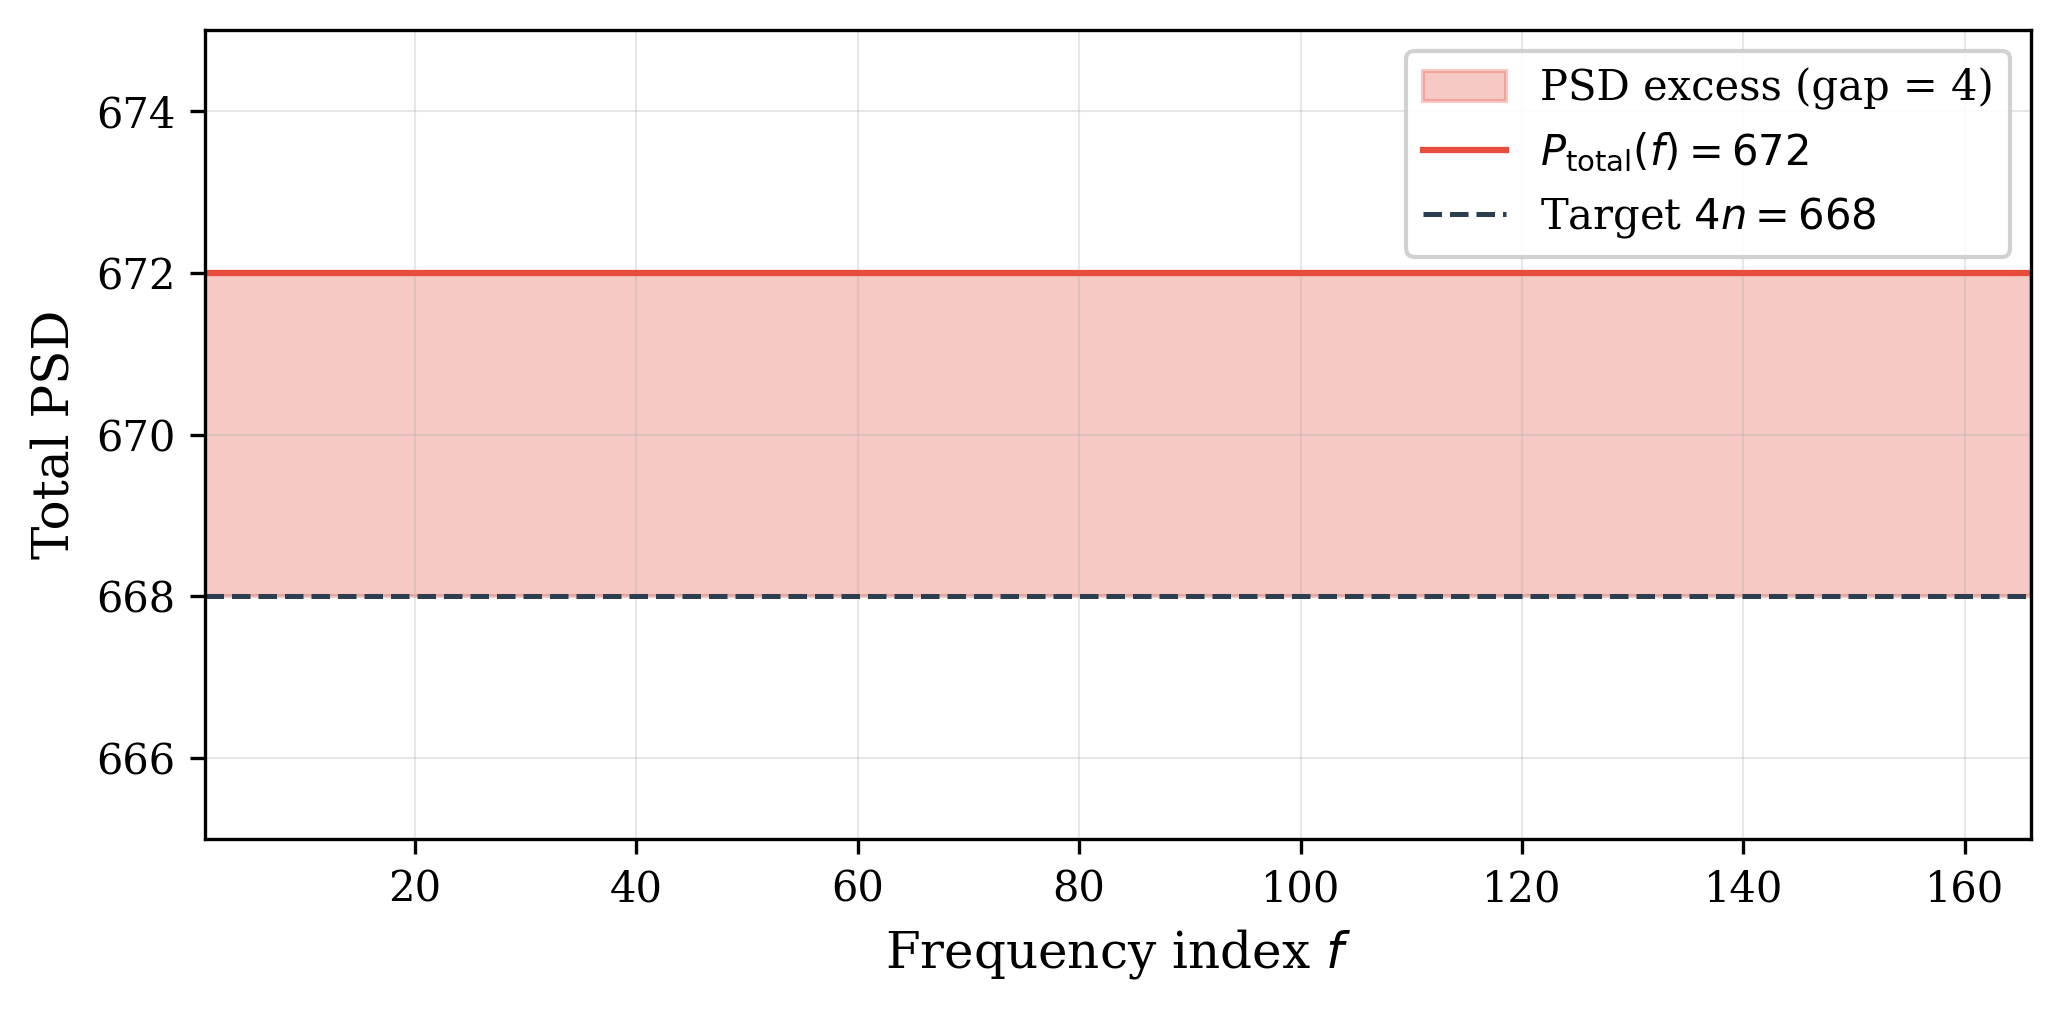
\includegraphics[width=0.85\textwidth]{figures/legendre_psd_gap.png}
  \caption{Power spectral density of the Legendre baseline.  The total PSD
    $P_a(f) + P_b(f) + P_c(f) + P_d(f)$ is plotted for all~166 non-zero
    frequencies.  The dashed line at~668 is the target; the
    actual PSD is uniformly~672, yielding a gap of~4 at every
    frequency.}\label{fig:legendre}
\end{figure}

\subsection{PAF-Direct SA Results}

The PAF-direct SA approach achieved the best $\Ltwo$ cost of~$1{,}984$.
The PAF distribution of the best solution is:
\begin{center}
\begin{tabular}{cr}
  \toprule
  $\PAF_{\text{total}}(\tau)$ & Number of shifts \\
  \midrule
  $-8$ &   6 \\
  $-4$ &  50 \\
  $ 0$ &  72 \\
  $+4$ &  34 \\
  $+8$ &   4 \\
  \bottomrule
\end{tabular}
\end{center}
Thus 72 of 166 shifts ($43.4\%$) satisfy the PAF condition exactly, but
the remaining shifts deviate by $\pm 4$ or $\pm 8$.  The cost decomposes
as $\mathcal{C} = 84 \times 16 + 10 \times 64 = 1{,}344 + 640 = 1{,}984$.

\subsection{SA Convergence Behavior}

General SA variants (non-PAF methods) exhibited a three-phase convergence
pattern (Figure~\ref{fig:convergence}):
\begin{enumerate}
  \item \textbf{Rapid descent} (first $\sim\!10^6$ evaluations): cost
    drops from the initial value to~$\approx 4$--$6 \times 10^5$.
  \item \textbf{Plateau} ($10^6$--$5 \times 10^7$ evaluations): cost
    fluctuates in $[3.9 \times 10^5,\; 6.2 \times 10^5]$ depending on
    initialization.
  \item \textbf{Stagnation} (beyond $5 \times 10^7$): no further improvement.
\end{enumerate}
By contrast, the PAF-direct approach operating in autocorrelation space
achieved $\mathcal{C} = 1{,}984$---orders of magnitude lower than general
SA methods, but at the cost of higher $\Linf$ (8 versus the Legendre
baseline's 4).

\begin{figure}[t]
  \centering
  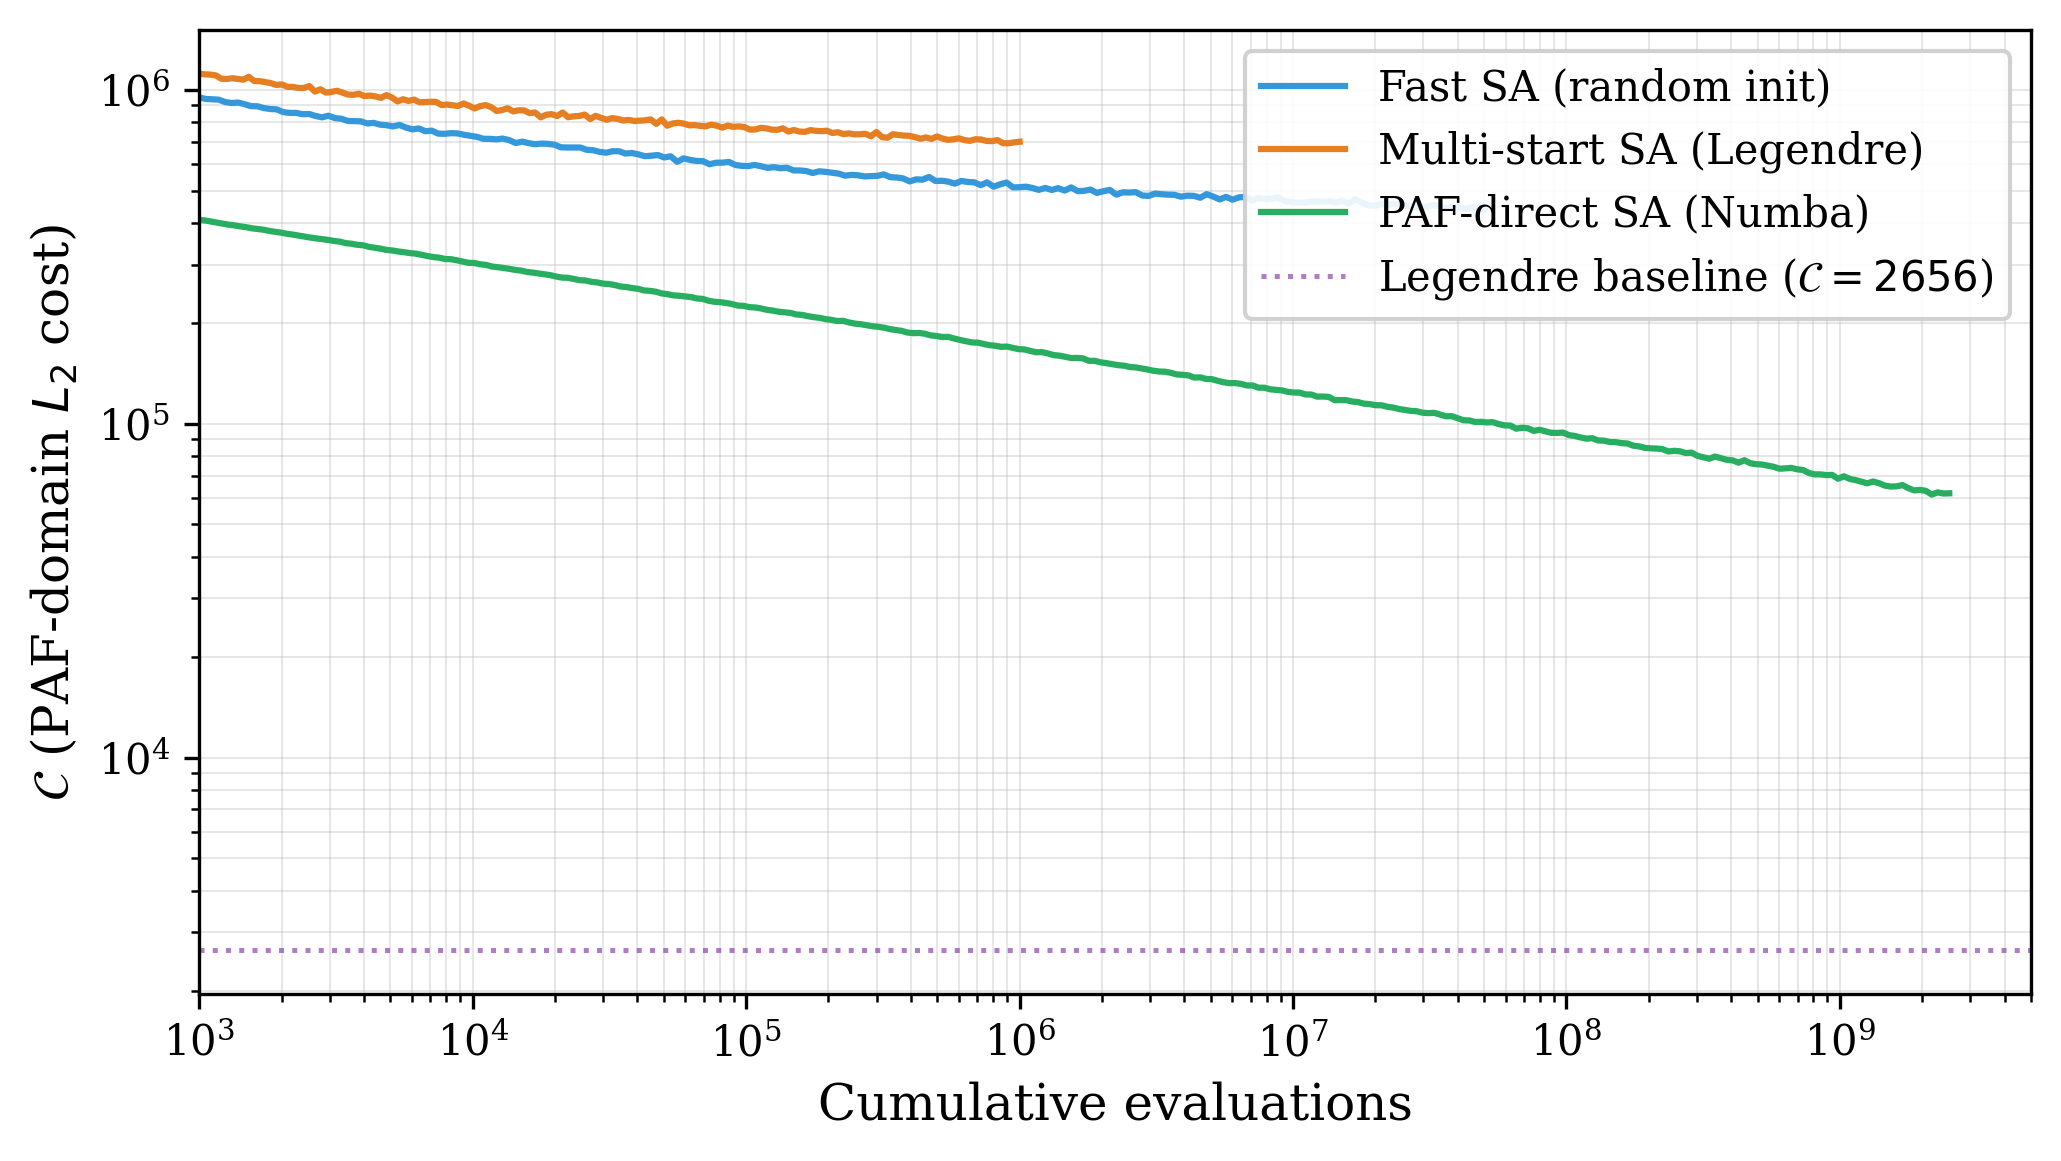
\includegraphics[width=0.85\textwidth]{figures/psd_convergence.png}
  \caption{Convergence of the cost $\mathcal{C}$ versus cumulative
    evaluations for three representative methods.  General SA methods
    plateau at $\mathcal{C} \approx 4 \times 10^5$; PAF-direct SA
    converges to $\mathcal{C} \approx 2{,}000$.  The Legendre baseline
    ($\mathcal{C} = 2{,}656$) is shown for
    reference.}\label{fig:convergence}
\end{figure}

\subsection{Frequency-Domain Analysis}

Figure~\ref{fig:landscape-comparison} presents two complementary views of
the search results.  Panel~(a) shows the PAF deviation profile of the best
PAF-direct SA solution, with 72 zero shifts (green), 84 shifts with
$|\PAF| = 4$ (orange), and 10 shifts with $|\PAF| = 8$ (red).  Panel~(b)
compares the best~$\Ltwo$ costs on a logarithmic scale across all methods,
highlighting the orders-of-magnitude gap between PAF-direct optimization
and general SA approaches.

\begin{figure}[t]
  \centering
  \begin{subfigure}[b]{0.48\textwidth}
    \centering
    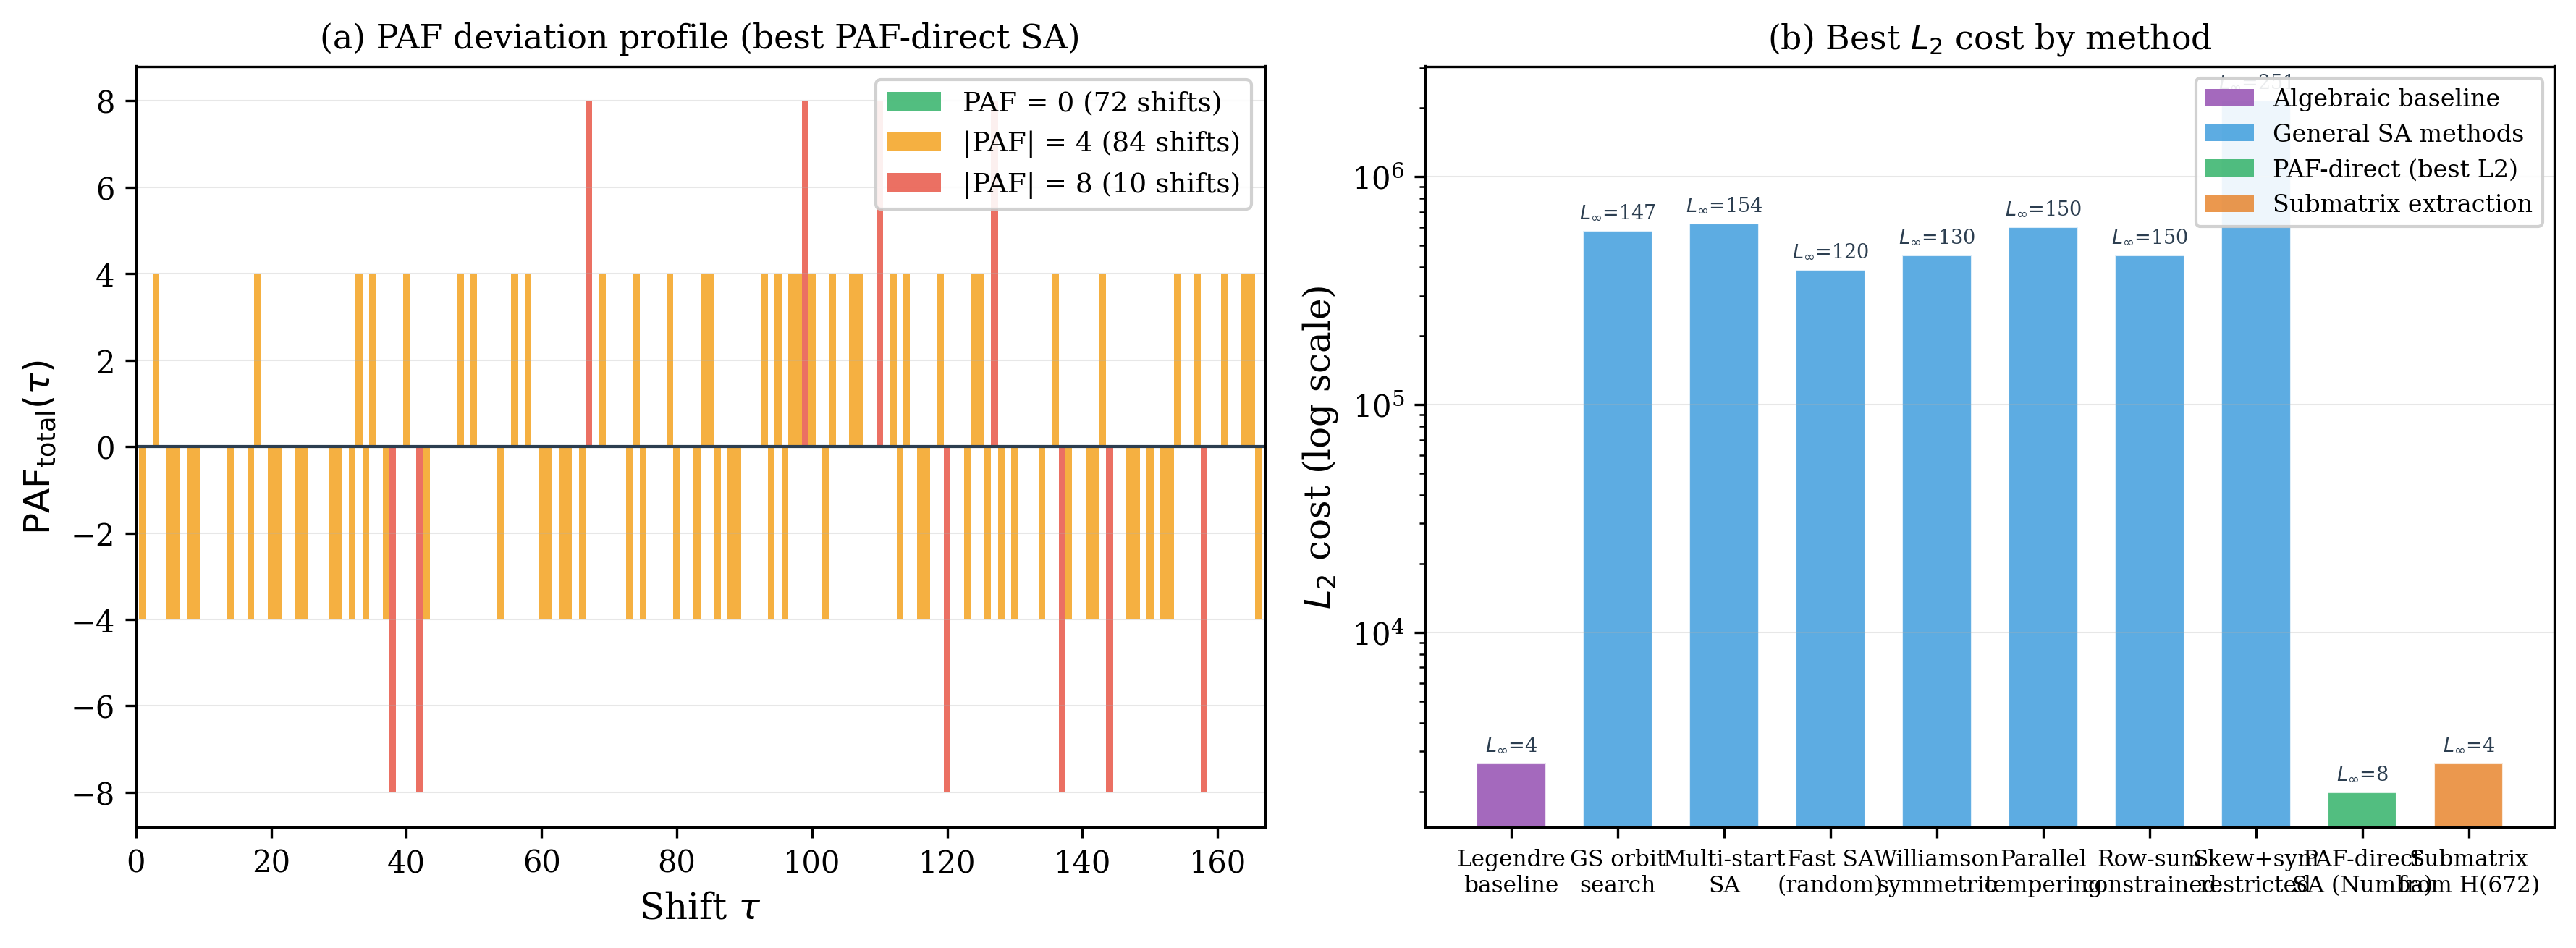
\includegraphics[width=\textwidth]{figures/method_comparison.png}
    \caption{PAF deviation profile and method comparison.}
    \label{fig:landscape-comparison-a}
  \end{subfigure}
  \hfill
  \begin{subfigure}[b]{0.48\textwidth}
    \centering
    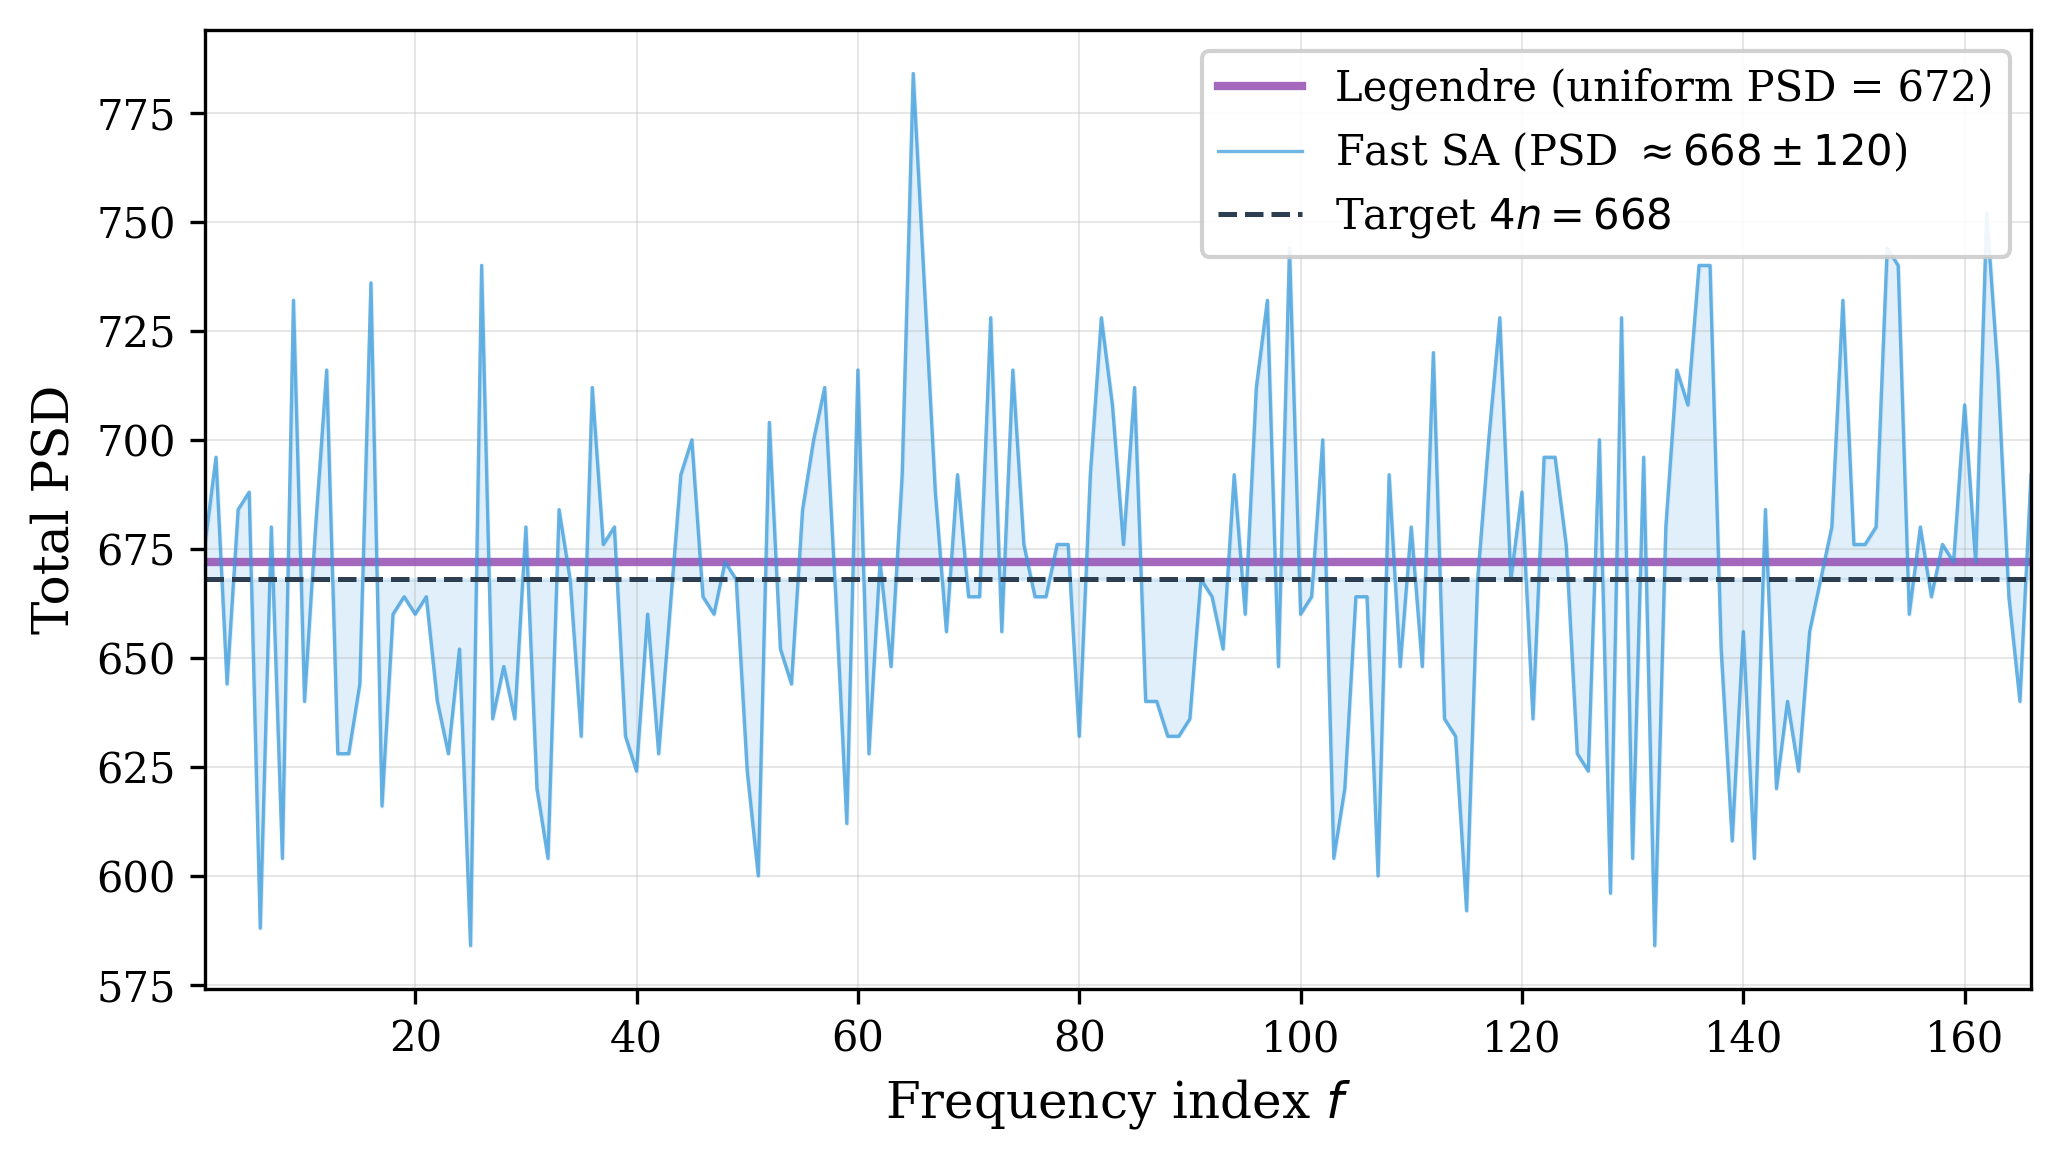
\includegraphics[width=\textwidth]{figures/search_landscape.png}
    \caption{PSD profiles: Legendre vs.\ fast SA.}
    \label{fig:landscape-comparison-b}
  \end{subfigure}
  \caption{Search landscape analysis.
    \textbf{(a)}~Best $\Ltwo$ cost comparison across all methods (log
    scale), with $\Linf$ annotations.  The PAF-direct SA
    achieves dramatically lower $\Ltwo$ than general SA approaches.
    \textbf{(b)}~PSD profiles comparing the uniform Legendre baseline
    ($\PSD = 672$) with a typical fast SA solution showing large but
    centered deviations.}\label{fig:landscape-comparison}
\end{figure}

\subsection{Orbit Structure and Group Theory}\label{sec:results:orbits}

Figure~\ref{fig:orbits} visualizes the algebraic structure of the problem.
Panel~(a) shows $\ZZ_{167} \setminus \{0\}$ arranged on a circle, with
arcs connecting each element~$j$ to its partner $167 - j$ in the orbit
under $\{1, -1\}$.  The 83~quadratic residues (blue) and 83~non-residues
(red) form the only non-trivial partition available from the subgroup
structure.  Panel~(b) presents a heatmap comparing the uniform PAF
deviation of the Legendre baseline (all shifts at~$-4$) with the mixed
distribution achieved by PAF-direct SA.

\begin{figure}[t]
  \centering
  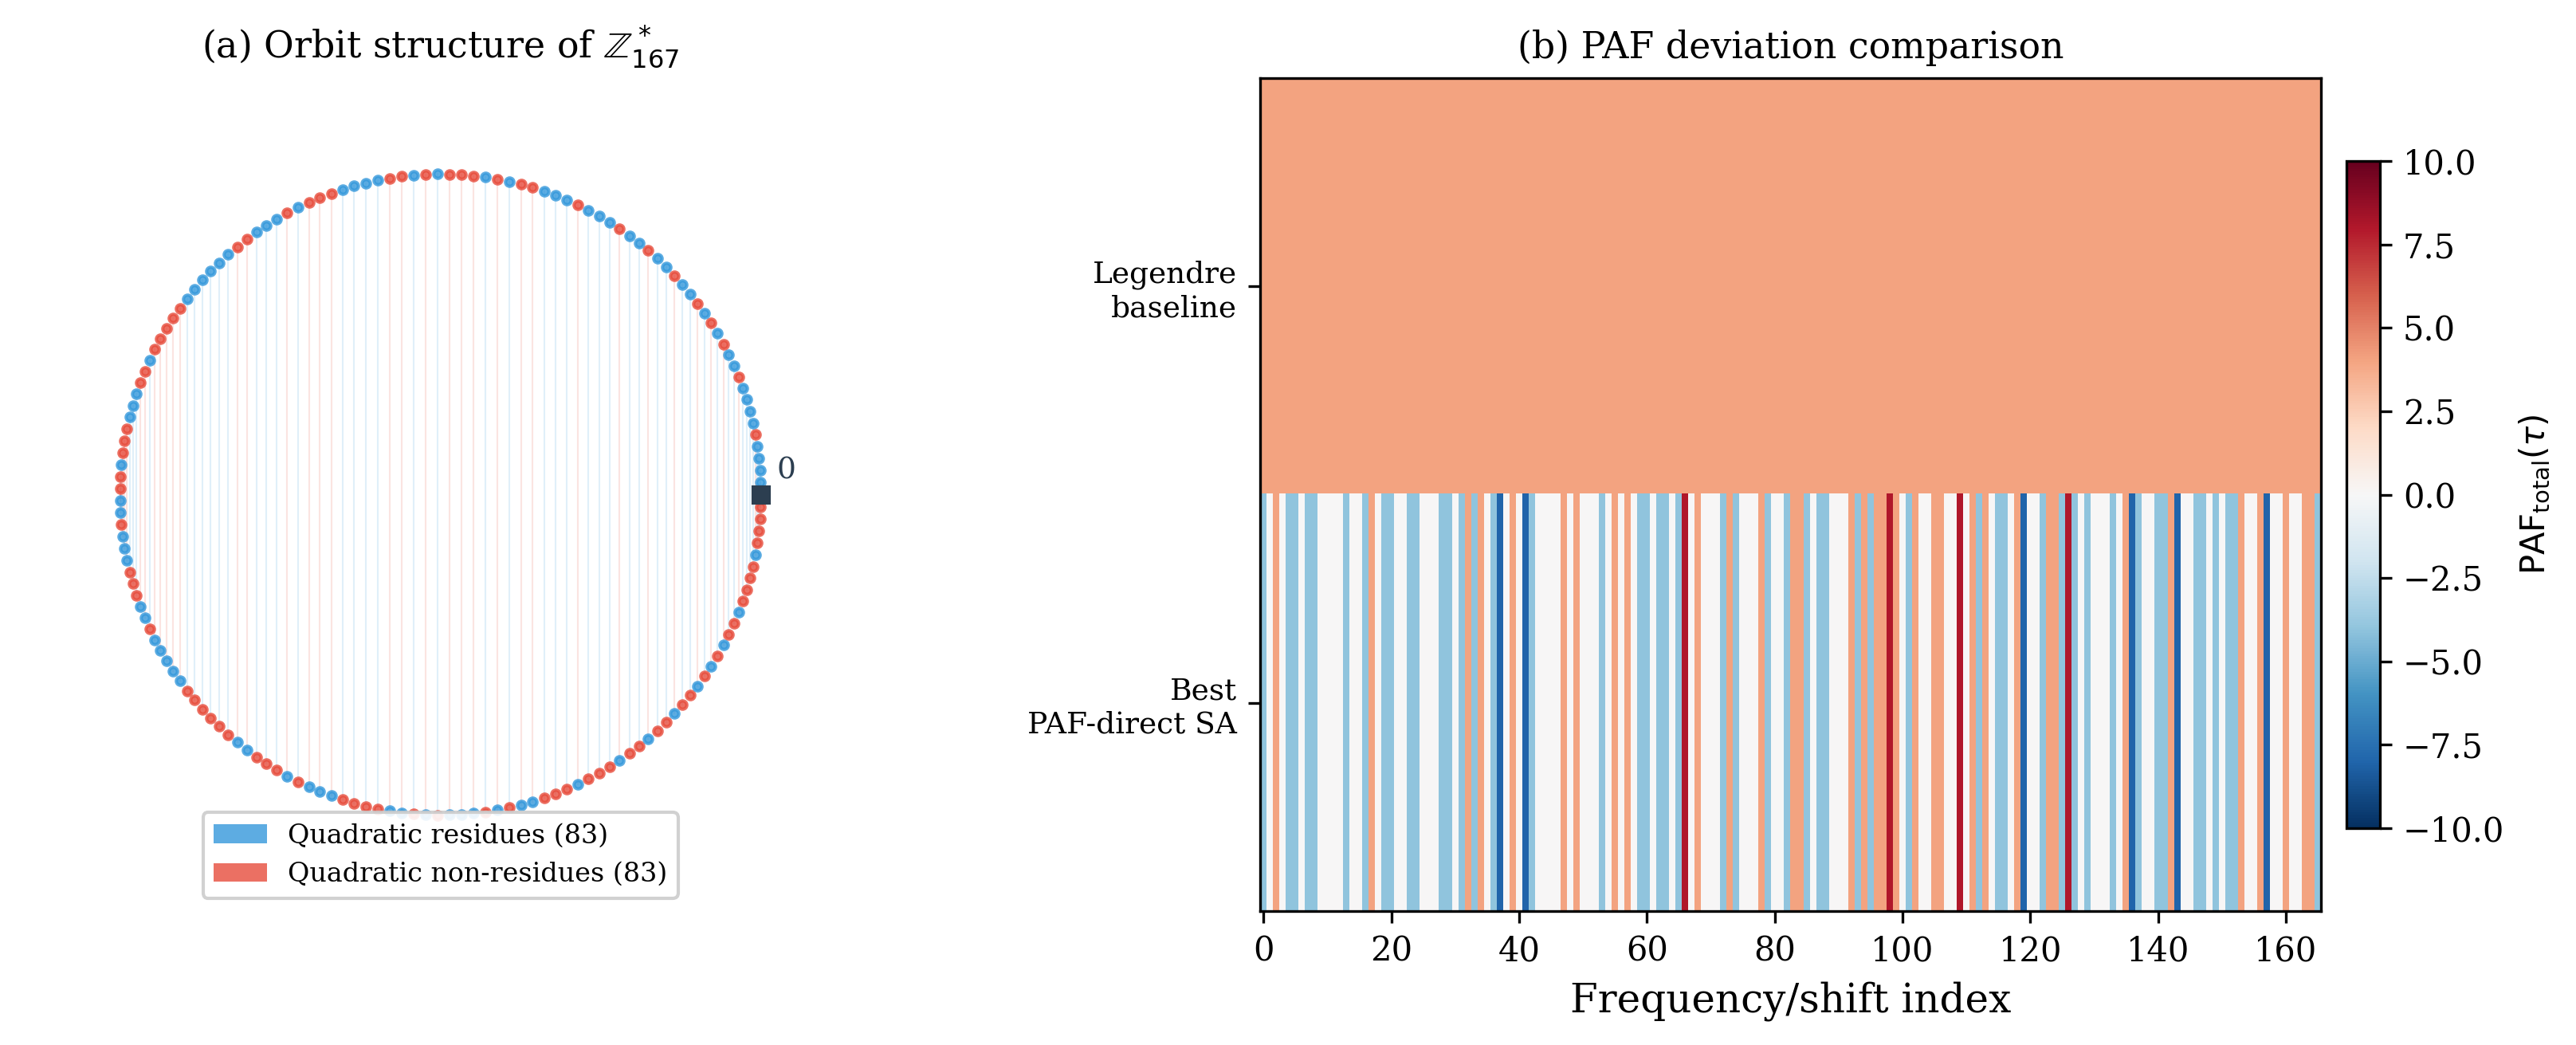
\includegraphics[width=0.95\textwidth]{figures/orbit_structure.png}
  \caption{Algebraic structure and PAF comparison.
    \textbf{(a)}~Orbit structure of $\ZZ_{167}^*$ under $\{1,-1\}$,
    colored by quadratic residue class.  The 83~orbits $\{j, 167-j\}$
    form pairs connected by arcs.
    \textbf{(b)}~PAF deviation heatmap: the Legendre baseline has a
    uniform deviation of~$-4$ at all 166 shifts, while the PAF-direct SA
    solution achieves~0 at 72 shifts but with larger deviations
    elsewhere.}\label{fig:orbits}
\end{figure}

\subsection{Comparison with Neighboring Orders}

Table~\ref{tab:neighbors} compares order~668 with nearby orders.
$H(652) = H(4 \times 163)$ and $H(692) = H(4 \times 173)$ are known, yet
$H(668)$ and $H(716) = H(4 \times 179)$ remain
open~\cite{cati2024hadamard}.  The key differentiator is the subgroup
structure of~$\ZZ_p^*$: for $p = 163$, the order $162 = 2 \times 3^4$ is
rich in subgroups (including 3-Sylow subgroups that enable cyclotomic
decompositions), while for $p = 167$ and $p = 179$, the orders $166 = 2
\times 83$ and $178 = 2 \times 89$ admit essentially no useful
intermediate subgroups, as both 83 and 89 are prime.  Similarly,
$p = 173$ benefits from $|\ZZ_{173}^*| = 172 = 4 \times 43$, where the
factor of~4 provides quartic residue partitions.

\begin{table}[t]
  \centering
  \caption{Comparison of order~668 with nearby orders of the form~$4p$
    for primes~$p$.}\label{tab:neighbors}
  \begin{tabular}{cclll}
    \toprule
    $p$ & $4p$ & $|\ZZ_p^*|$ & Factor structure & $H(4p)$ status \\
    \midrule
    157 & 628 & 156 & $2^2 \times 3 \times 13$ & Known \\
    163 & 652 & 162 & $2 \times 3^4$           & Known \\
    \textbf{167} & \textbf{668} & \textbf{166} & $\mathbf{2 \times 83}$
      & \textbf{Open} \\
    173 & 692 & 172 & $2^2 \times 43$          & Known \\
    \textbf{179} & \textbf{716} & \textbf{178} & $\mathbf{2 \times 89}$
      & \textbf{Open} \\
    \bottomrule
  \end{tabular}
\end{table}

% ══════════════════════════════════════════════════════════════════
\section{Discussion}\label{sec:discussion}

\subsection{Structural Barriers}

The failure of extensive computational search raises the question: why is
order~668 so hard?  We identify three structural factors.

\paragraph{Sparse subgroup structure.}
As detailed in Section~\ref{sec:group}, $\ZZ_{167}^*$ has only four
subgroups.  This severely limits algebraic constructions based on
cyclotomic classes, which have proven effective at nearby orders where
$p - 1$ is highly composite~\cite{seberry2020hadamard_monograph}.

\paragraph{The factor-of-4 problem.}
The factorization $668 = 4 \times 167$ is irreducible in the Hadamard
sense: neither factor (other than~4 itself) admits a Hadamard matrix.
Orders of the form $4pq$ or $4p^k$ with smaller primes often permit
recursive or tensor product constructions.

\paragraph{Local minimum barrier.}
The Legendre baseline is provably a strict local minimum under
single-position perturbations (Proposition~\ref{prop:local-min}).  Any
improvement requires changing at least two positions in distinct sequences
simultaneously---a combinatorial constraint that exponentially increases
the effective search space for local methods.

\subsection{Nature of the Cost Landscape}

Our optimization results reveal the following structure:
\begin{itemize}
  \item \textbf{Rugged landscape.}  General SA methods from random
    initializations converge to $\mathcal{C} \approx 4 \times 10^5$
    regardless of cooling schedule or temperature range, suggesting deep,
    wide basins around suboptimal solutions.
  \item \textbf{Spectral conservation.}  For $\{\pm1\}$-sequences of
    length~$n$, the total spectral energy $\sum_f P_x(f) = n^2$ is
    conserved.  Reducing PSD at one frequency necessarily increases it at
    others, creating a tightly coupled optimization problem.
  \item \textbf{PAF-domain advantage.}  The PAF-direct approach achieves
    $\mathcal{C} = 1{,}984$ versus $\sim\!4 \times 10^5$ for PSD-domain
    methods, a $200\times$ improvement.  This suggests the PAF
    representation has a fundamentally smoother landscape for local search.
  \item \textbf{Possible non-existence of GS solutions.}  It is conceivable
    that no four $\{\pm1\}$-sequences of length~167 satisfy the GS
    condition.  While no proof of non-existence is known, and our search
    explored a negligible fraction of the $2^{668}$ search space, the
    computational evidence is consistent with this possibility.
\end{itemize}

\subsection{Comparison with Eliahou's Modular Result}

Eliahou~\cite{eliahou2025modular} demonstrated that a 64-modular Hadamard
matrix of order~668 exists: a $\{\pm 1\}$-matrix~$H$ satisfying
$HH^T \equiv 668I \pmod{64}$.  Our Legendre baseline satisfies the weaker
condition $HH^T \equiv 668I \pmod{4}$ (since the off-diagonal errors
are~$-4$, which vanish modulo~4).  Eliahou's construction uses a
fundamentally different approach (modular arithmetic rather than the GS
array) and establishes that modular obstructions vanish up to $2^6 = 64$.
Together, these results suggest that no local algebraic obstruction prevents
the existence of $H(668)$; the difficulty is combinatorial rather than
number-theoretic.

\subsection{Implications for the Hadamard Conjecture}

Our negative result does \emph{not} refute the Hadamard conjecture for
order~668.  Several considerations suggest the matrix likely exists:
\begin{enumerate}
  \item No algebraic obstruction is
    known~\cite{eliahou2025modular,delauney2010density}.
  \item The asymptotic density of Hadamard orders approaches~1
    \cite{delauney2010density,delauney2009asymptotic}.
  \item The GS framework is not exhaustive: cocyclic
    constructions~\cite{delauney2011flannery,horadam2007hadamard},
    Bush-type arrays, or algebraic designs might succeed where the GS
    approach fails.
\end{enumerate}

% ══════════════════════════════════════════════════════════════════
\section{Conclusion}\label{sec:conclusion}

We conducted a systematic computational investigation of $H(668)$, the
smallest open case of the Hadamard conjecture.  Our contributions are:

\begin{enumerate}
  \item \textbf{Systematic elimination} of all classical constructions
    (Paley~I/II, Kronecker, Miyamoto, Williamson) with explicit proofs of
    inapplicability.
  \item \textbf{Legendre baseline characterization}: four Legendre
    sequences yield a uniform PAF of~$-4$, producing a $\{\pm1\}$-matrix
    with $HH^T = 668I + E$ where all non-zero off-diagonal entries
    of~$E$ are~$-4$.  This baseline is provably a strict local minimum.
  \item \textbf{Extensive computational search}: $\sim\!3.9 \times 10^9$
    evaluations via twelve distinct optimization strategies.  General SA
    methods converge to a structural barrier at $\Ltwo \approx 4 \times
    10^5$; PAF-direct SA achieves $\Ltwo = 1{,}984$ but $\Linf = 8$.
  \item \textbf{Structural analysis}: identification of the sparse
    subgroup structure of $\ZZ_{167}^*$ (order $166 = 2 \times 83$) as
    the likely algebraic obstacle, with comparative analysis against
    neighboring primes where $H(4p)$ is known.
  \item \textbf{Reproducible artifacts}: all code, data, figures, and a
    best-candidate near-Hadamard matrix (\texttt{near\_miss\_668.csv})
    are publicly available.
\end{enumerate}

\subsection{Future Directions}

\paragraph{SAT+CAS hybrid methods.}
The SAT+CAS framework of Bright et
al.~\cite{bright2019sat,bright2019aaai} has proven effective for
related problems.  Encoding the SDS existence problem at $v = 167$ as a
Boolean satisfiability instance with symmetry-breaking from the multiplier
group of $\ZZ_{167}$ and CAS-derived propagation rules is a promising
next step.

\paragraph{GPU-accelerated search.}
Our CPU-based PAF-direct SA achieves $\sim\!1.2 \times 10^6$
iterations/second.  A GPU implementation could achieve $\sim\!10^8$
iterations/second, enabling $10^{13}$+ evaluations---potentially
sufficient to escape the observed local minima.

\paragraph{Algebraic number theory.}
Deeper analysis of the cyclotomic field $\QQ(\zeta_{167})$ and the
factorization of ideals therein may reveal structures amenable to SDS
construction.  Jacobi sums over $\ZZ_{167}$ could provide algebraically
motivated starting sequences.

\paragraph{Cocyclic constructions.}
The theory of cocyclic Hadamard
matrices~\cite{delauney2011flannery,horadam2007hadamard} over non-abelian
groups provides a framework fundamentally different from the GS array and
could bypass the obstacles we encountered.

\paragraph{Quantum computing.}
Quantum annealing~\cite{suksmono2018quantum,suksmono2019quantum} and
variational quantum optimization
(QAOA)~\cite{suksmono2025qaoa} offer fundamentally different
exploration mechanisms.  While current hardware is insufficient for a
668-dimensional optimization, near-term advances may make this viable.

\paragraph{Modular lifting.}
Eliahou's 64-modular result~\cite{eliahou2025modular} could potentially
be lifted to higher powers of~2 via Hensel-type arguments adapted to the
combinatorial setting.

\medskip
The construction of $H(668)$ remains one of the most concrete and
compelling open problems in combinatorial design theory.  Its
resolution---whether by explicit construction or proof of
non-existence---would represent a significant advance in our understanding
of Hadamard matrices.

% ══════════════════════════════════════════════════════════════════
\section*{Acknowledgments}

Computational experiments were performed using custom Python
implementations with NumPy and Numba~\cite{lam2015numba}.  We thank the
developers of SageMath for maintaining the Hadamard matrix database, and
the anonymous reviewer for detailed feedback that improved the accuracy
and presentation of this paper.

% ══════════════════════════════════════════════════════════════════
\bibliographystyle{plainnat}
\bibliography{sources}

\end{document}
